\documentclass[11pt]{article}
\usepackage{amsmath}
\usepackage{graphicx}
\usepackage{hyperref}
\usepackage{enumitem}
\usepackage{geometry}
\geometry{a4paper, margin=0.75in}

\title{Developing a Data-Driven Platform for Enhanced Cattle Farm Management: Anomaly Detection, Analytics, and Simulation}
\author{Kevin George}
\date{July 16, 2024}

\begin{document}

\begin{titlepage}
    \centering
    \vspace*{0.3in}
    \LARGE\textbf{Thesis Proposal: Developing a Data-Driven Platform for Enhanced Cattle Farm Management: Anomaly Detection, Analytics, and Simulation}\par
    \vspace{0.5in}
    \large Kevin George\par
    \vspace{0.2in}
    \normalsize July 16, 2024
    \thispagestyle{empty}
\end{titlepage}

\section*{1. Motivation}
Advancing smart agriculture through the use of real sensor data is crucial for improving farm management, animal welfare, and resource optimization. By focusing on cattle farms, this research aims to leverage sensor data to enhance operations, ensure animal welfare, and manage resources more effectively, facilitating smarter decision-making.


\section*{2. Problem Statement}

Modern cattle farming faces significant challenges in resource management, animal welfare, and operational efficiency. Existing data management solutions often lack the advanced analytics and monitoring capabilities needed to support effective decision-making. These limitations include high costs, compatibility issues with farm-specific devices, and insufficient integration with advanced data collection technologies.

Our proposed platform seeks to address these issues by integrating with the WeideInsight system, utilizing technologies such as Bluetooth Low Energy (BLE) and mioty for precise data collection. This platform is designed to provide comprehensive, data-driven decision-making tools tailored specifically for cattle farming. It distinguishes itself from existing platforms like \textbf{Digitanimal}, \textbf{Performance Livestock Analytics (PLA)}, \textbf{Livestocked}, \textbf{NAVFARM}, \textbf{Farm Manager and Analyzer}, \textbf{AGEX Herd}, \textbf{Ranch Manager}, and \textbf{ThingsBoard} by offering specialized, cost-effective features that meet the unique requirements of this sector.

\textbf{Research Question:} How can a data-driven platform be developed to enhance decision-making in cattle farm management through advanced monitoring, analytics, and simulation capabilities?

\section*{3. Related Fields}
\begin{itemize}
    \item \textbf{Precision Agriculture:} Techniques and technologies aimed at monitoring and managing variability in crops and livestock, including the use of advanced sensors and data analytics for precise farm management.
    \item \textbf{Sensors and Communication Technologies:} The application of sensors for data collection, including temperature, humidity, and livestock tracking. Technologies like Bluetooth Low Energy (BLE) and mioty enable efficient data transmission, with BLE suited for short-range, low-power use, and mioty for long-range, low-energy transmission.
    \item \textbf{Big Data Analytics:} Utilization of large datasets collected from sensors to extract meaningful insights, trends, and patterns. This includes optimizing farm management practices and improving decision-making processes based on data analysis.
    \item \textbf{Machine Learning:} The use of machine learning algorithms for predictive modeling, anomaly detection, and decision support, particularly in monitoring livestock health and activity.
    \item \textbf{Semantic Web and Ontologies:} Employment of semantic models and ontologies to integrate and interpret diverse data sources in agriculture, enhancing data interoperability and providing a comprehensive understanding of agricultural systems.
\end{itemize}

\section*{4. Approach}
The proposed system architecture comprises several interlinked components, each fulfilling a specific role in data management and analytics for cattle farming. The flow and interaction among these components are detailed below:

\begin{enumerate}[label=\arabic*., wide=0pt, left=0pt]

    \item \textbf{Data Ingestion Component:} The collected data from Weidelnsight via API and then ingested by the Data Ingestion Component. This Component aggregates data from various sources, ensuring it is ready for processing and analysis.

    \item \textbf{Centralized Data Platform in University:}
    \begin{itemize}
        \item \textbf{Postgres Database Component:} Data is stored in the Postgres Database Component, which acts as a central repository. It supports efficient data querying and transactions, forming the backbone for data management.
        \item \textbf{Common Resource (Data Management) Component:} This Component oversees the central storage and management of both raw and processed data, ensuring schema consistency and data integrity.
    \end{itemize}

    \item \textbf{Analytic Reporting and Processing:}
    \begin{itemize}
        \item \textbf{Analytic Engine Component:} The Analytic Engine Component processes the stored data, running machine learning models and statistical analyses. It generates actionable insights, predictions, and recommendations based on the analysis.
        \item \textbf{Watcher/Pattern Recognition Component:} This component continuously monitors data streams to identify anomalies and patterns. It plays a crucial role in predictive analytics and anomaly detection.
        \item \textbf{Alert Engine Component:} Based on predefined rules and detected anomalies, this Component generates alerts and notifications. It manages the distribution of these alerts through appropriate channels.
    \end{itemize}

    \item \textbf{User Interaction and Integration:}
    \begin{itemize}
        \item \textbf{User Interface Component:} This component provides web and mobile interfaces, allowing users to interact with the system. It handles user authentication, authorization, and presents data visualizations and dashboards.
        \item \textbf{Gateway Service:} Acting as an API gateway, the Gateway Service routes client requests to the appropriate microservices, managing API rate limiting, security, and load balancing.
        \item \textbf{Service Registry and Discovery Service:} This service maintains a registry of all available system services, enabling them to register and discover each other.
        \item \textbf{SmartSPEC Simulation Component:} For scenario analysis, the SmartSPEC Simulation Component integrates real-time and historical data. It provides simulation capabilities to validate model accuracy and assess system robustness under different conditions.
    \end{itemize}
\end{enumerate}
\begin{figure}[h!]
    \centering
    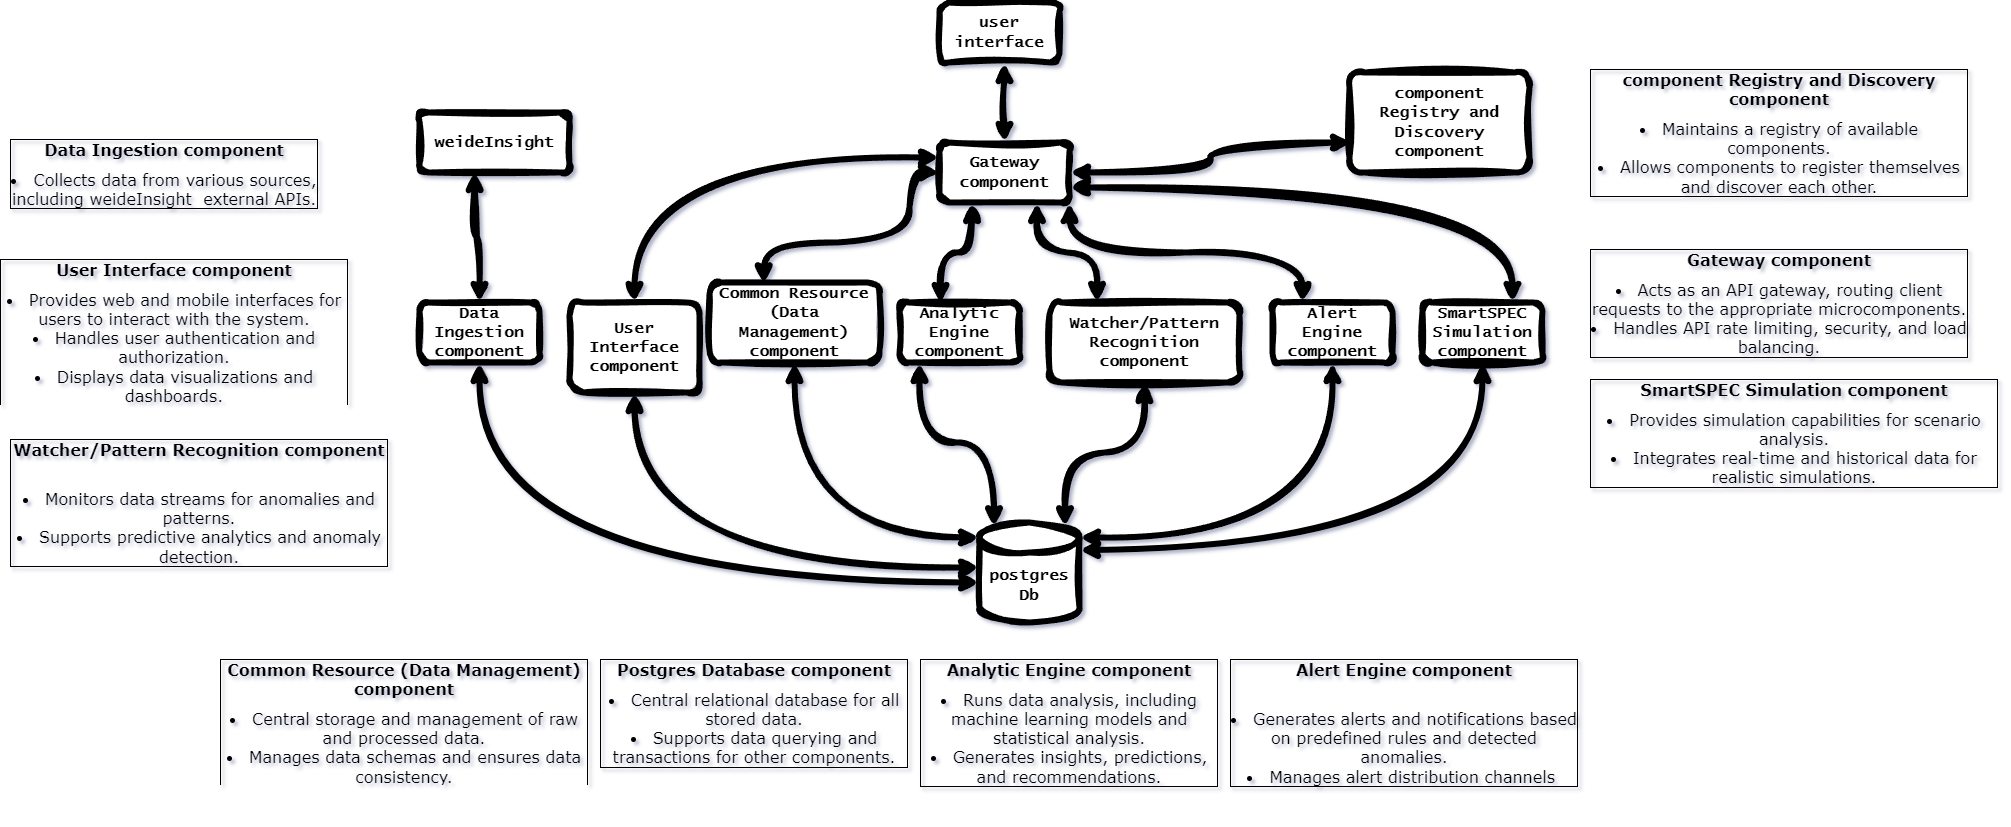
\includegraphics[width=\textwidth]{archite.png}
    \caption{Proposed Architecture for the Data-Driven Agricultural Decision Making Platform}
    \label{fig:architecture}
\end{figure}

\section*{5. Evaluation}
\textbf{Experiments:} Use real sensor data from cattle farms and simulated data generated using SmartSPEC to evaluate:
\begin{itemize}
    \item \textbf{Pattern and Anomaly Detection:} Assess the effectiveness of methods in detecting patterns and anomalies in both real and simulated data, utilizing semantic models to enhance interpretation.
    \item \textbf{Analytic Reporting:} Evaluate the efficacy of analytic tools in deriving actionable insights from real and simulated data.
    \item \textbf{Comparison with Related Work:} Compare performance against existing solutions using both real and simulated data.
    \item \textbf{Expected Results:} Achieve enhanced data quality and better decision-making supported by both real-world and simulated data.
\end{itemize}



\section*{6. Expected Outcomes}
The research is expected to deliver a comprehensive platform for real-time livestock monitoring, enhanced data analytics, and reliable anomaly detection. The platform will facilitate improved decision-making in cattle farming through precise data management and insightful reporting.

\section*{7. Project Timeline}
\begin{itemize}
    \item \textbf{August:} Literature review and data collection. Begin drafting the introduction and literature review sections.
    \item \textbf{September:} Development and testing of pattern recognition and anomaly detection methods. Document methodology and initial findings.
    \item \textbf{October:} Implementation of analytic tools and integration of semantic models. Document implementation details and findings.
    \item \textbf{November:} Integration of simulation components and evaluation of platform performance. Document evaluation and draft the conclusion and discussion sections.
    \item \textbf{December:} Finalize the thesis, including proofreading, editing, and preparing for the defense. Ensure thesis is submission-ready.
\end{itemize}



\section*{8. Related Work}
\begin{enumerate}[label=\arabic*., wide=0pt, left=0pt]
    \item \textbf{Chio, A., et al.} "SmartSPEC: Customizable Smart Space Datasets via Event-driven Simulations." \textit{IEEE International Conference on Pervasive Computing and Communications (PerCom)}. This paper discusses the creation of customizable datasets, integrating simulation with real-world data for applications in smart agriculture. [1]
    
    \item \textbf{Pongratz, P.} "A Simulator for Location-Based Agriculture Scenarios." Master's Thesis, University of Bamberg. This thesis details the development of a simulator that uses location-based data in conjunction with SmartSPEC to model agricultural scenarios. [2]
    
    \item \textbf{Jares, D.} "Simulating Hybrid Location Models for Smart Agriculture Demonstrators." Master's Thesis, University of Bamberg. This work explores the challenges and solutions associated with simulating hybrid location models in smart agriculture, including the integration of actual data to extend previous work. [3]
    
    \item \textbf{Sundararajan, S. S., et al.} "Big Data Analytics for Smart Farming." \textit{Big Data Journal}. This article examines techniques in big data analytics relevant to agriculture, providing a foundation for the development of analytics tools for smart farming. [4]
    
    \item \textbf{Alimi, A. M., et al.} "Machine Learning for Anomaly Detection in Agriculture." \textit{Applied Sciences}. This paper explores the use of machine learning techniques to detect anomalies in agricultural data, focusing on enhancing the reliability and efficiency of agricultural operations. [5]
    
    \item \textbf{Smith, J., et al.} "Semantic Models in Agriculture: Enhancing Data Integration and Quality." \textit{International Journal of Semantic Computing}. This paper discusses the role of semantic models in improving the integration and quality of data in agricultural applications. [6]
\end{enumerate}

\section*{9. References}
\begin{thebibliography}{9}
\bibitem{Chio} Chio, A., et al. SmartSPEC: Customizable Smart Space Datasets via Event-driven Simulations. \textit{IEEE International Conference on Pervasive Computing and Communications (PerCom)}.

\bibitem{Pongratz} Pongratz, P. A Simulator for Location-Based Agriculture Scenarios. Master's Thesis, University of Bamberg.

\bibitem{Jares} Jares, D. Simulating Hybrid Location Models for Smart Agriculture Demonstrators. Master's Thesis, University of Bamberg.

\bibitem{Sundararajan} Sundararajan, S. S., et al. Big Data Analytics for Smart Farming. \textit{Big Data Journal}.

\bibitem{Alimi} Alimi, A. M., et al. Machine Learning for Anomaly Detection in Agriculture. \textit{Applied Sciences}.

\bibitem{Smith} Smith, J., et al. Semantic Models in Agriculture: Enhancing Data Integration and Quality. \textit{International Journal of Semantic Computing}.
\end{thebibliography}

\end{document}
